\documentclass[a4paper]{article}
\usepackage[utf8]{vntex}
\usepackage[english]{babel}
\usepackage[utf8]{inputenc}
\usepackage{amsmath,graphicx,xcolor,booktabs,array,indentfirst}
\usepackage[margin=25mm,headheight=28pt,headsep=8mm]{geometry}
\usepackage{fancyhdr,listings}
\usepackage[colorlinks=true,linkcolor=black,citecolor=black,urlcolor=blue]{hyperref}
\setlength{\parindent}{1cm}
\setlength{\parskip}{0pt}
\setlength{\emergencystretch}{2em}
\raggedbottom
\clubpenalty=10000
\widowpenalty=10000
\pagestyle{fancy}
\fancyhf{}
\fancyhead[L]{\small Ho Chi Minh City University of Technology\\
Faculty of Computer Science and Engineering}
\fancyfoot[L]{\footnotesize Microprocessors--Microcontrollers Laboratory (CO3010)}
\fancyfoot[R]{\footnotesize\thepage}
\renewcommand{\headrulewidth}{0.3pt}
\definecolor{codeblue}{RGB}{0,83,160}
\definecolor{codebg}{RGB}{247,248,250}
\lstset{language=C,basicstyle=\ttfamily\small,
keywordstyle=\color{codeblue}\bfseries,stringstyle=\color{red!60!black},
numbers=left,numberstyle=\tiny\color{gray},numbersep=7pt,
frame=single,rulecolor=\color{gray!40},backgroundcolor=\color{codebg},
breaklines=true,breakatwhitespace=false,keepspaces=true,
columns=fullflexible,tabsize=4,showstringspaces=false,
captionpos=t,aboveskip=10pt,belowskip=10pt,xleftmargin=12pt,
framexleftmargin=3pt}
\newcommand{\code}[1]{\texttt{\detokenize{#1}}}
\newcommand{\topic}[1]{\subsection{#1}}
\begin{document}
\hypersetup{pageanchor=false}
\begin{titlepage}
\centering
{\large VIETNAM NATIONAL UNIVERSITY HO CHI MINH CITY\par}
\vspace{3mm}
{\large HO CHI MINH CITY UNIVERSITY OF TECHNOLOGY\par}
\vspace{3mm}
{\large FACULTY OF COMPUTER SCIENCE AND ENGINEERING\par}
\vspace{15mm}

\includegraphics[width=4cm]{hcmut_logo.png}\par
\vspace{13mm}
\par{\Large\bfseries Microprocessors--Microcontrollers Laboratory\par}
{\Large\bfseries (CO3010)\par}
\vspace{8mm}
\rule{\textwidth}{0.5pt}\par
\vspace{6mm}
{\Large\bfseries Laboratory Report\par}
\vspace{6mm}
{\LARGE\bfseries LAB 02\par}
\vspace{4mm}
{\Large\bfseries Timer Interrupt and LED Scanning\par}
\vspace{6mm}
\rule{\textwidth}{0.5pt}\par
\vspace{18mm}
\begin{tabular}{rl}
Advisor: & Phan Văn Sỹ\\[3mm]
Student: & Nguyễn Cáp Quốc Khánh\\[3mm]
Student ID: & 2452500\\[3mm]
Class: & CC03
\end{tabular}
\vfill
{\small HO CHI MINH CITY, OCTOBER 2026\par}
\end{titlepage}
\hypersetup{pageanchor=true}
\pagenumbering{roman}
\begingroup
\small
\tableofcontents
\endgroup
\clearpage
\listoffigures
\listoftables
\clearpage
\pagenumbering{arabic}
\section*{Overview}
\addcontentsline{toc}{section}{Overview}
Timer interrupts provide a periodic timing source for display control. Rather than
using a separate delay for every output, one hardware timer can supply a common
tick from which several intervals are obtained. The STM32F103 combines timer
peripherals and general-purpose outputs suitable for these tasks\cite{stm32}.

Seven-segment multiplexing connects corresponding segment terminals together
and enables one digit at a time. The selected digit receives its segment pattern
for a fixed time slot before the next digit is selected. This reduces the number
of GPIO signals required for a multi-digit display. A digital clock separates
timekeeping from display conversion: hours and minutes are converted into four
decimal digits, while scanning repeatedly selects their physical displays.

Software timers use counters to count hardware ticks and flags to indicate
expiry. Independent timers allow clock updates, DOT transitions, and display
selection to run at different intervals. Moving application processing into the
main loop keeps the interrupt routine short. The same approach extends to an
eight-column LED matrix, where column patterns form a character and changing
the buffer creates animation.

STM32CubeMX provides peripheral configuration, Keil \mbox{$\mu$Vision} provides
the firmware development environment\cite{keil}, and Proteus provides circuit
schematic and simulation tools\cite{proteus}. HAL functions provide the timer
and GPIO interfaces used throughout the exercises\cite{hal}.

\topic{Hardware timing base}
The system uses the internal 8 MHz HSI clock without a PLL. AHB and APB1 are
undivided, so TIM2 receives 8 MHz. Its prescaler is 7999 and its auto-reload
value is 9. Since both divisions include zero, the timing is
\begin{align*}
f_{\mathrm{counter}}&=\frac{8\,000\,000}{7999+1}=1000\ \mathrm{Hz},\\
f_{\mathrm{interrupt}}&=\frac{1000}{9+1}=100\ \mathrm{Hz},\\
T_{\mathrm{interrupt}}&=\frac{1}{100}=10\ \mathrm{ms}.
\end{align*}
Thus, 50 interrupts represent 500 ms, 25 represent 250 ms, and 100 represent
1000 ms. Enable the TIM2 global interrupt and start the timer in interrupt
mode after initialization. The HAL callback is invoked for each update event;
it is not itself an infinite loop\cite{hal}.
\par\noindent\begin{minipage}{\linewidth}
\begin{lstlisting}[caption={Essential TIM2 settings and start operation}]
htim2.Instance = TIM2;
htim2.Init.Prescaler = 7999;
htim2.Init.CounterMode = TIM_COUNTERMODE_UP;
htim2.Init.Period = 9;
HAL_TIM_Base_Start_IT(&htim2);
\end{lstlisting}
\end{minipage}\par
These lines identify the required settings and start operation; the timer start
belongs after the generated peripheral initialization and application setup.
Each exercise is a separate program version. A replacement callback or main
loop replaces its earlier version. Shared helpers are retained unless a change
is explicitly described.

\section{Exercise 1: Two-digit scanning}
\topic{Implementation idea and circuit}
The design uses time sharing because both displays are connected to the same
seven segment signals. If both common anodes were enabled together, both
digits would receive the same numeral. Therefore, the program selects only
one display at a time and alternates between them. The shared segment outputs
determine the numeral, while the enable outputs determine its physical position.

The objective is to display 1 on the first common-anode digit and 2 on the
second, changing the selected digit every 500 ms. Segments a--g share PB0--PB6.
PA6 and PA7 control the PNP enable circuits. A low enable output turns its
transistor on, and a low segment output lights the corresponding segment.
Before changing the pattern, both digits are disabled so that the previous
digit does not receive the next digit's data.
For example, numeral 1 requires segments b and c, whereas numeral 2 requires
a, b, d, e, and g. The same PB0--PB6 outputs must consequently carry different
patterns in the two display slots. The PNP transistors provide the common-anode
selection: their bases are pulled low to enable the associated display and
high to disable it.
\begin{figure}[htbp]
\centering
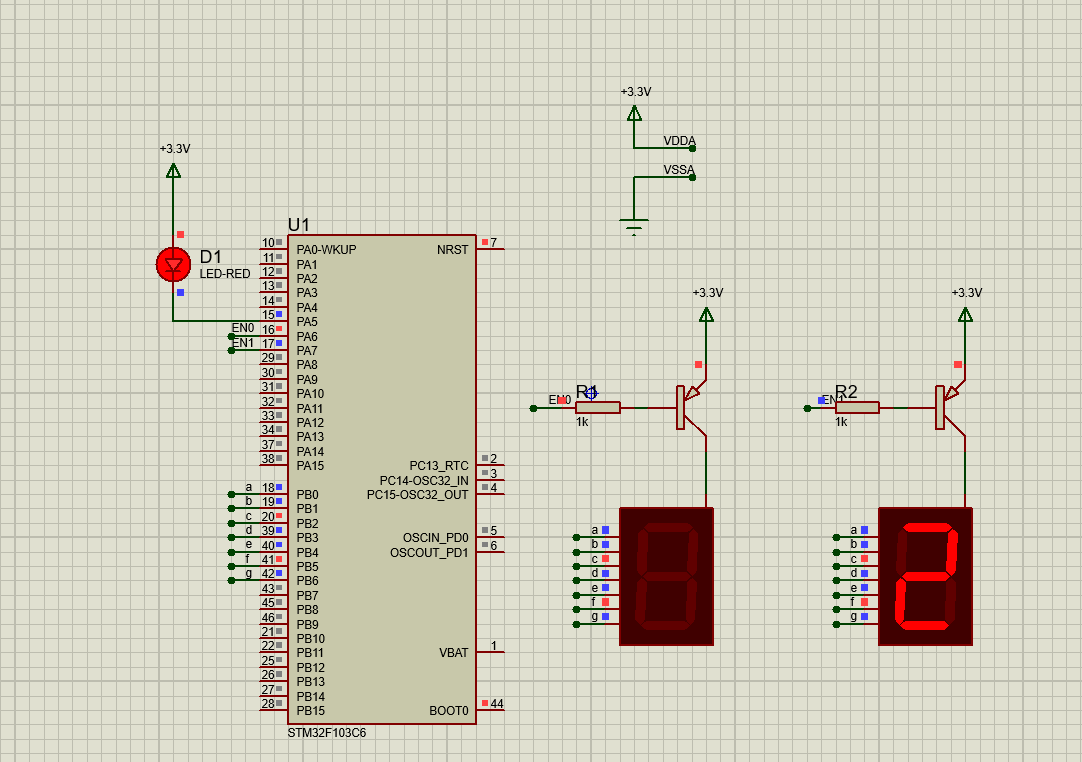
\includegraphics[width=0.92\textwidth]{ex1.png}
\caption{Exercise 1: two common-anode displays with shared segment signals.}
\label{fig:ex1}
\end{figure}

\topic{Shared segment function}
The lookup table stores the segment pins required for each decimal numeral.
First all segments are set high, then the required segments are driven low.
An invalid input leaves the segments blank. This function is reused in all
seven-segment exercises.
\par\noindent\begin{minipage}{\linewidth}
\begin{lstlisting}[caption={Segment definitions and decimal conversion}]
#define LED_A GPIO_PIN_0
#define LED_B GPIO_PIN_1
#define LED_C GPIO_PIN_2
#define LED_D GPIO_PIN_3
#define LED_E GPIO_PIN_4
#define LED_F GPIO_PIN_5
#define LED_G GPIO_PIN_6
#define ALL_LEDS (LED_A | LED_B | LED_C | LED_D | \
                  LED_E | LED_F | LED_G)

void display7SEG(int num)
{
    static const uint16_t digit[10] =
    {
        LED_A | LED_B | LED_C | LED_D | LED_E | LED_F,
        LED_B | LED_C,
        LED_A | LED_B | LED_D | LED_E | LED_G,
        LED_A | LED_B | LED_C | LED_D | LED_G,
        LED_B | LED_C | LED_F | LED_G,
        LED_A | LED_C | LED_D | LED_F | LED_G,
        LED_A | LED_C | LED_D | LED_E | LED_F | LED_G,
        LED_A | LED_B | LED_C,
        LED_A | LED_B | LED_C | LED_D | LED_E | LED_F | LED_G,
        LED_A | LED_B | LED_C | LED_D | LED_F | LED_G
    };

    HAL_GPIO_WritePin(GPIOB, ALL_LEDS, GPIO_PIN_SET);
    if (num >= 0 && num <= 9)
    {
        HAL_GPIO_WritePin(GPIOB, digit[num], GPIO_PIN_RESET);
    }
}
\end{lstlisting}
\end{minipage}\par

\topic{Interrupt implementation and scanning frequency}
Before starting TIM2, disable PA6 and PA7, display 1, and enable PA6.
The callback counts 50 ticks before exchanging the selected display.
The two static variables retain their values between callback invocations.
The threshold follows directly from the required switching time:
\[
N_{\mathrm{ticks}}=\frac{500\ \mathrm{ms}}{10\ \mathrm{ms}}=50.
\]
The callback returns after each interrupt. The hardware timer continues to
count, and another callback invocation occurs at the next tick. This means
the 500-ms interval is accumulated over 50 short invocations rather than by
waiting inside one callback.

At each expiry, \code{counter} is reset to zero and \code{led_index} is
changed using \code{1 - led_index}. This expression maps zero to one and one
to zero, so no separate wrapping condition is needed for two positions. Both
enables are then driven high, the next segment pattern is written, and only
the chosen enable is driven low. Disabling the displays before changing data
prevents a short unwanted numeral during the transition.
\par\noindent\begin{minipage}{\linewidth}
\begin{lstlisting}[caption={Two-digit timer callback}]
void HAL_TIM_PeriodElapsedCallback(TIM_HandleTypeDef *htim)
{
    static uint8_t counter = 0;
    static uint8_t led_index = 0;

    if (htim->Instance == TIM2)
    {
        counter++;
        if (counter >= 50)
        {
            counter = 0;
            led_index = 1 - led_index;
            HAL_GPIO_WritePin(GPIOA, GPIO_PIN_6 | GPIO_PIN_7,
                              GPIO_PIN_SET);
            if (led_index == 0)
            {
                display7SEG(1);
                HAL_GPIO_WritePin(GPIOA, GPIO_PIN_6,
                                  GPIO_PIN_RESET);
            }
            else
            {
                display7SEG(2);
                HAL_GPIO_WritePin(GPIOA, GPIO_PIN_7,
                                  GPIO_PIN_RESET);
            }
        }
    }
}
\end{lstlisting}
\end{minipage}\par
The digit selection changes twice per second. However, a complete scan includes
both digits:
\[
T_{\mathrm{scan}}=2\times500\ \mathrm{ms}=1\ \mathrm{s},\qquad
f_{\mathrm{scan}}=1\ \mathrm{Hz}.
\]
Each digit has a nominal 50\% duty cycle. At this deliberately slow rate, the
expected output is visibly alternating digits rather than a steady two-digit
image.
With digit 0 selected at startup, the expected sequence is digit 0 from
0 to 500 ms, digit 1 from 500 to 1000 ms, and digit 0 again from 1000 to
1500 ms. Thus, a particular physical digit is selected once per second even
though a selection change occurs every half second.

\section{Exercise 2: Four-digit multiplexing}
\topic{Implementation idea and circuit extension}
The idea is to extend the two-position scanner into a circular four-position
scanner. One index selects the active digit, while an array stores the four
numerals. Two independent counters are maintained from the same 10-ms
interrupt: one changes the selected digit and the other changes the DOT state.
This permits the display and DOT to operate at different periods without an
additional hardware timer.

The four positions need only seven shared segment outputs and four enable
outputs. DOT adds one control signal. The program can therefore control the
four numerals and the central LEDs using twelve signals rather than four
independent groups of segment outputs. Each selected display remains active
until its slot expires; the other three common anodes stay disabled.

Four displays share PB0--PB6, while PA6--PA9 select their common anodes.
The two central LEDs share PA4, labeled DOT, and therefore change state together.
The buffer contains \code{{1, 2, 3, 0}}, representing 12:30. The circuit in
Figure~\ref{fig:ex2} is reused through Exercise 8.
\begin{figure}[htbp]
\centering
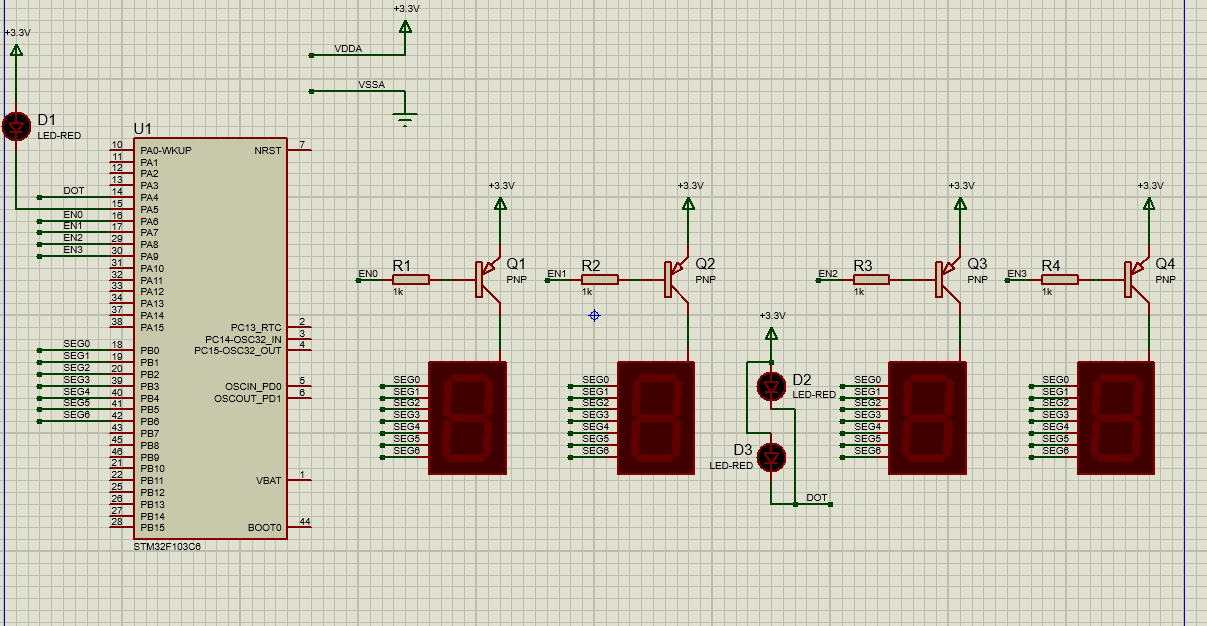
\includegraphics[width=\textwidth]{ex2.png}
\caption{Exercise 2: four multiplexed digits and the DOT output.}
\label{fig:ex2}
\end{figure}
\par\noindent\begin{minipage}{\linewidth}
\begin{lstlisting}[caption={Four-digit definitions and selection helper}]
#define EN0 GPIO_PIN_6
#define EN1 GPIO_PIN_7
#define EN2 GPIO_PIN_8
#define EN3 GPIO_PIN_9
#define ALL_EN (EN0 | EN1 | EN2 | EN3)
#define DOT_PIN GPIO_PIN_4
#define MAX_LED 4
#define TIMER_CYCLE 10

int led_buffer[MAX_LED] = {1, 2, 3, 0};
int index_led = 0;
static const uint16_t enable_pin[MAX_LED] =
{
    EN0, EN1, EN2, EN3
};

void disable7SEG(void)
{
    HAL_GPIO_WritePin(GPIOA, ALL_EN, GPIO_PIN_SET);
}

void update7SEG(int index)
{
    if (index < 0 || index >= MAX_LED)
    {
        return;
    }
    disable7SEG();
    display7SEG(led_buffer[index]);
    HAL_GPIO_WritePin(GPIOA, enable_pin[index], GPIO_PIN_RESET);
}
\end{lstlisting}
\end{minipage}\par

\topic{Independent countdowns}
Timer0 supplies the 1000-ms DOT interval and timer1 supplies the 500-ms digit
interval. Each setter converts milliseconds into 10-ms ticks and clears its
expiry flag. The flag becomes one only when a positive counter reaches zero.
The following functions are reused in Exercises 3--8.
The initial counter values are calculated separately:
\[
C_{\mathrm{DOT}}=\frac{1000}{10}=100,\qquad
C_{\mathrm{digit}}=\frac{500}{10}=50.
\]
Both counters decrease on every TIM2 update, but neither counter is derived
from the other. Consequently, changing the digit interval does not change the
DOT interval. The setters reload a countdown and clear its old expiry flag.
Without clearing the flag, a completed event would continue to satisfy the
callback's condition on later ticks.
\par\noindent\begin{minipage}{\linewidth}
\begin{lstlisting}[caption={Two simple software timers}]
int timer0_counter = 0;
int timer0_flag = 0;
int timer1_counter = 0;
int timer1_flag = 0;

void setTimer0(int duration)
{
    timer0_counter = duration / TIMER_CYCLE;
    timer0_flag = 0;
}

void setTimer1(int duration)
{
    timer1_counter = duration / TIMER_CYCLE;
    timer1_flag = 0;
}

void timer_run(void)
{
    if (timer0_counter > 0)
    {
        timer0_counter--;
        if (timer0_counter == 0)
        {
            timer0_flag = 1;
        }
    }
    if (timer1_counter > 0)
    {
        timer1_counter--;
        if (timer1_counter == 0)
        {
            timer1_flag = 1;
        }
    }
}
\end{lstlisting}
\end{minipage}\par
Initialize the first digit and both timers before starting TIM2. Setting
\code{index_led = 1} records that digit 0 is already selected.
\par\noindent\begin{minipage}{\linewidth}
\begin{lstlisting}[caption={Four-digit application initialization}]
disable7SEG();
update7SEG(0);
index_led = 1;
setTimer0(1000);
setTimer1(500);
HAL_TIM_Base_Start_IT(&htim2);
\end{lstlisting}
\end{minipage}\par
\par\noindent\begin{minipage}{\linewidth}
\begin{lstlisting}[caption={Four-digit timer callback}]
void HAL_TIM_PeriodElapsedCallback(TIM_HandleTypeDef *htim)
{
    if (htim->Instance == TIM2)
    {
        timer_run();
        if (timer0_flag == 1)
        {
            HAL_GPIO_TogglePin(GPIOA, DOT_PIN);
            setTimer0(1000);
        }
        if (timer1_flag == 1)
        {
            update7SEG(index_led);
            index_led++;
            if (index_led >= MAX_LED)
            {
                index_led = 0;
            }
            setTimer1(500);
        }
    }
}
\end{lstlisting}
\end{minipage}\par
The index follows 0, 1, 2, 3, then returns to 0. The main loop needs no display
processing at this stage. Each digit is selected for 500 ms, giving
\[
T_{\mathrm{scan}}=4\times500\ \mathrm{ms}=2\ \mathrm{s},\qquad
f_{\mathrm{scan}}=0.5\ \mathrm{Hz}.
\]
Digit selection still changes at 2 Hz, but each digit is revisited at 0.5 Hz
with a nominal 25\% duty cycle. DOT toggles every second, so one complete
ON--OFF cycle lasts two seconds and has frequency 0.5 Hz.

\topic{Execution sequence}
The initial call to \code{update7SEG(0)} displays the first buffer element,
which is 1. The next index is set to one because position zero has already
been prepared. After 50 ticks, position one displays 2. After another 50
ticks, position two displays 3 and DOT changes state because its 100-tick
countdown also expires. The callback checks both flags separately, so neither
event prevents the other from being processed.

The remaining positions are selected in the same manner. At 1500 ms,
position three displays 0. At 2000 ms, the index returns to zero and DOT
changes state again. The buffer is fixed during this exercise, so the
expected output represents 12:30 while the digit enables cycle continuously.
At the selected low frequency, the active positions remain visibly separate.

\section{Exercise 3: Buffer-based digit selection}
\topic{Implementation idea and selection function}
The implementation separates \emph{what is displayed} from \emph{where it is
displayed}. The array \code{led_buffer} holds the four numerals, whereas
\code{index_led} identifies the physical digit to enable. Therefore, later
exercises can change clock data inside the buffer without changing the GPIO
selection algorithm. For example, index two identifies the third physical
display; its numeral is read from \code{led_buffer[2]} and need not equal two.
This distinction is essential when the buffer later represents clock digits.

The buffer is \code{{1, 2, 3, 4}}, and a switch-based selector replaces the
array-based enable lookup from Exercise 2. The circuit and segment helper
remain unchanged. Each case performs two operations: convert the selected
buffer value into a segment pattern and enable its associated display.
The \code{break} statement ends that case so another display is not enabled
by falling through into the next case.
\par\noindent\begin{minipage}{\linewidth}
\begin{lstlisting}[caption={Switch-based update7SEG function}]
int led_buffer[MAX_LED] = {1, 2, 3, 4};

void update7SEG(int index)
{
    disable7SEG();
    switch (index)
    {
        case 0:
            display7SEG(led_buffer[0]);
            HAL_GPIO_WritePin(GPIOA, EN0, GPIO_PIN_RESET);
            break;
        case 1:
            display7SEG(led_buffer[1]);
            HAL_GPIO_WritePin(GPIOA, EN1, GPIO_PIN_RESET);
            break;
        case 2:
            display7SEG(led_buffer[2]);
            HAL_GPIO_WritePin(GPIOA, EN2, GPIO_PIN_RESET);
            break;
        case 3:
            display7SEG(led_buffer[3]);
            HAL_GPIO_WritePin(GPIOA, EN3, GPIO_PIN_RESET);
            break;
        default:
            break;
    }
}
\end{lstlisting}
\end{minipage}\par
An invalid index selects no digit because all enables are disabled before the
switch. The callback retains the Exercise 2 timing while using the new
selection function:
\par\noindent\begin{minipage}{\linewidth}
\begin{lstlisting}[caption={Exercise 3 timer callback}]
void HAL_TIM_PeriodElapsedCallback(TIM_HandleTypeDef *htim)
{
    if (htim->Instance == TIM2)
    {
        timer_run();
        if (timer0_flag == 1)
        {
            HAL_GPIO_TogglePin(GPIOA, DOT_PIN);
            setTimer0(1000);
        }
        if (timer1_flag == 1)
        {
            update7SEG(index_led);
            index_led++;
            if (index_led >= MAX_LED)
            {
                index_led = 0;
            }
            setTimer1(500);
        }
    }
}
\end{lstlisting}
\end{minipage}\par

\topic{Buffer substitution and expected behavior}
With the original buffer, the scan selects numerals 1, 2, 3, and 4. A useful
buffer check replaces those values with \code{{4, 3, 2, 1}}: the expected sequence
then becomes 4, 3, 2, and 1 without changing the scanner. Similarly,
\code{{0, 0, 0, 0}} should select zero at every position. These examples check
the distinction between the digit index and its stored numeral.

The index must remain between 0 and 3; otherwise the scanner leaves all digits
disabled. The timing remains 500 ms per digit, 2 s per complete scan, and
0.5 Hz for the four-digit scan. Buffer conversion can therefore change later
without rewriting the selection logic.

To follow one scan, the initialization first calls \code{update7SEG(0)},
which reads buffer value 1 and selects EN0. At the next expiry, index one
reads value 2 and selects EN1. Subsequent expiries select EN2 and EN3 with
values 3 and 4. Incrementing the index after each call makes it refer to the
next position. When it reaches four, the wrapping condition restores zero
before the next selection.

The function changes the GPIO state only for the requested position; it does
not contain a delay or advance the scan by itself. Scheduling remains the
callback's responsibility. With four 500-ms slots, a complete frame still
takes 2000 ms. Buffer substitution changes the content of those slots, while
the timing and nominal 25\% duty cycle remain the same.

\section{Exercise 4: One-hertz display scanning}
\topic{Implementation idea and timing calculation}
The circuit and selection function are unchanged. Only the software-timer
duration assigned to each digit is recalculated. A complete scan must last
one second; because four digits receive equal slots, each digit must remain
selected for one quarter of that period. Setting a one-second delay for each
digit would produce a four-second scan, so the required complete-frame period
must first be divided by the number of displays.

For four equally timed displays, the general relationship and selected values
are
\[
T_{\mathrm{slot}}=\frac{1}{Nf_{\mathrm{scan}}}
=\frac{1}{4\times1}=0.25\ \mathrm{s},\qquad
C_{\mathrm{slot}}=\frac{250}{10}=25.
\]
Timer1 is therefore rearmed with 250 instead of 500. Timer0 remains at 1000 ms
because the DOT transition interval is unchanged. Digit selection occurs at
4 Hz, while the complete scan occurs at 1 Hz.

\topic{Replacement timer callback}
The Exercise 3 switch function and buffer are retained. The callback becomes:
\par\noindent\begin{minipage}{\linewidth}
\begin{lstlisting}[caption={One-hertz four-digit scanning callback}]
void HAL_TIM_PeriodElapsedCallback(TIM_HandleTypeDef *htim)
{
    if (htim->Instance == TIM2)
    {
        timer_run();
        if (timer0_flag == 1)
        {
            HAL_GPIO_TogglePin(GPIOA, DOT_PIN);
            setTimer0(1000);
        }
        if (timer1_flag == 1)
        {
            update7SEG(index_led);
            index_led++;
            if (index_led >= MAX_LED)
            {
                index_led = 0;
            }
            setTimer1(250);
        }
    }
}
\end{lstlisting}
\end{minipage}\par
In the initial setup, use \code{setTimer1(250)}. After \code{update7SEG(0)},
set \code{index_led = 1}. This avoids selecting digit 0 twice at startup;
leaving its index at zero would make its initial active interval 500 ms.
The steady sequence has four 250-ms slots and a nominal 25\% duty cycle per
digit. The low scan frequency makes the selection order visible.

\topic{Expected scan and independent DOT timing}
Starting with position zero already selected, the next positions become active
at approximately 250, 500, and 750 ms. At 1000 ms, position zero is selected
again, completing the first full frame. This gives four selection events per
second and one complete frame per second. Short GPIO switching operations
are ignored in these nominal timing calculations.

The DOT counter still contains 100 ticks, so it expires once for every four
25-tick digit slots. On that expiry, the callback both toggles DOT and selects
the next digit. The two tasks continue independently because the same hardware
tick updates two separate countdowns. Reducing the digit interval improves
the complete scan rate from 0.5 Hz to 1 Hz without speeding up DOT.

\section{Exercise 5: Digital clock and decimal buffer}
\topic{Implementation idea and clock representation}
The clock is divided into three responsibilities. The variables \code{hour},
\code{minute}, and \code{second} preserve time; \code{updateClockBuffer()}
converts hours and minutes into four decimal digits; and the scanner from
Exercise 4 displays those digits. This separation means that a carry from
seconds to minutes changes only the data buffer and does not alter the scanning
procedure.

Only hours and minutes are visible, but seconds must still be maintained to
determine when a minute has elapsed. One displayed minute therefore corresponds
to 60 time-update operations. Keeping time as three integer variables also
makes the rollover rules explicit: seconds and minutes range from 0 to 59,
and hours range from 0 to 23.

The four displays represent HH:MM. Hours, minutes, and seconds are maintained
as integer variables initialized to 15, 8, and 50. Seconds determine when the
minute changes but are not displayed. Replace the static numeral buffer with
\code{{0, 0, 0, 0}} and initialize it from the current time.

The first two positions contain the hour tens and units, and the last two
contain the minute tens and units. Division by 10 extracts the tens digit;
the remainder after division by 10 extracts the units digit.
\par\noindent\begin{minipage}{\linewidth}
\begin{lstlisting}[caption={Clock variables and updateClockBuffer function}]
int hour = 15;
int minute = 8;
int second = 50;
int led_buffer[MAX_LED] = {0, 0, 0, 0};

void updateClockBuffer(void)
{
    led_buffer[0] = hour / 10;
    led_buffer[1] = hour % 10;
    led_buffer[2] = minute / 10;
    led_buffer[3] = minute % 10;
}
\end{lstlisting}
\end{minipage}\par
For 15:08, integer division gives \(15/10=1\) and \(8/10=0\), while the
remainders are 5 and 8. The zero is therefore inserted automatically.
More generally, each value \(x\) in the clock range can be expressed as
\[
x=10q+r,\qquad q=\left\lfloor\frac{x}{10}\right\rfloor,
\qquad r=x\bmod10.
\]
The quotient supplies the tens position and the remainder supplies the units
position. For a one-digit value, the quotient is zero, so the same computation
handles leading zeros without a special branch. Each resulting buffer entry
is between zero and nine and can be passed to \code{display7SEG()}.
\begin{table}[htbp]
\centering
\caption{Expected clock-to-buffer conversion}
\label{tab:clock}
\begin{tabular}{ccccc}
\toprule
Time & Hour tens & Hour units & Minute tens & Minute units\\
\midrule
15:08 & 1 & 5 & 0 & 8\\
09:05 & 0 & 9 & 0 & 5\\
00:00 & 0 & 0 & 0 & 0\\
23:59 & 2 & 3 & 5 & 9\\
\bottomrule
\end{tabular}
\end{table}

\topic{Blocking time update and rollover}
The main loop in this exercise waits one second before advancing the clock.
The callback remains the Exercise 4 callback, so interrupts continue to scan
digits and toggle DOT while the foreground waits.
The delay is placed before the increment, so the initial value 15:08:50 is
kept for the first one-second interval. Each subsequent iteration advances
time once and refreshes the HH:MM buffer. The foreground waits during
\code{HAL_Delay()}, but TIM2 still provides the interrupt-driven display
timing used in Exercise 4.
\par\noindent\begin{minipage}{\linewidth}
\begin{lstlisting}[caption={Exercise 5 main loop}]
while (1)
{
    HAL_Delay(1000);
    second++;
    if (second >= 60)
    {
        second = 0;
        minute++;
    }
    if (minute >= 60)
    {
        minute = 0;
        hour++;
    }
    if (hour >= 24)
    {
        hour = 0;
    }
    updateClockBuffer();
}
\end{lstlisting}
\end{minipage}\par
The ordered checks propagate the carry from seconds to minutes and then to
hours. Expected transitions include 15:08:59 to 15:09:00, 15:59:59 to 16:00:00,
and 23:59:59 to 00:00:00. Call \code{updateClockBuffer()} before selecting the
first digit, initialize \code{index_led = 1}, and arm timers at 1000 and 250 ms.

For reuse in the following exercises, the time-update statements are placed
in a helper without changing their behavior:
\par\noindent\begin{minipage}{\linewidth}
\begin{lstlisting}[caption={Reusable one-second clock update}]
void updateClock(void)
{
    second++;
    if (second >= 60)
    {
        second = 0;
        minute++;
    }
    if (minute >= 60)
    {
        minute = 0;
        hour++;
    }
    if (hour >= 24)
    {
        hour = 0;
    }
    updateClockBuffer();
}
\end{lstlisting}
\end{minipage}\par
The conversion function changes data only; the scanner still selects one
digit every 250 ms. A complete scan remains one second, regardless of the
current clock value.

\topic{Rollover example and expected display}
Consider the last second of a day. Starting at 23:59:59, incrementing seconds
produces 60. The first condition changes seconds to zero and increments minutes
to 60. The second condition then changes minutes to zero and increments hours
to 24. Finally, the third condition restores hours to zero. All three checks
must occur during the same time-update operation so the final state is
00:00:00 rather than an intermediate out-of-range time.

At startup, \code{updateClockBuffer()} stores \code{{1, 5, 0, 8}} before the
first display is enabled. During seconds 51 through 59, the HH:MM buffer
remains the same because neither the hour nor the minute has changed. On the
tenth update after 15:08:50, the time reaches 15:09:00 and the buffer becomes
\code{{1, 5, 0, 9}}. The scanner continues its 250-ms slots throughout these
updates, showing how timekeeping and display selection perform different jobs.

\section{Exercise 6: Software-timer operation}
\topic{Implementation idea, counter, and flag}
The main idea is to represent a requested delay by a remaining number of
10-ms ticks. The software-timer part of the interrupt routine decreases
counters and raises expiry flags. The main program observes a flag, performs the corresponding action,
and rearms that timer. This structure allows the processor to continue other
work while a delay is in progress.

A software timer represents a delay by counting periodic interrupts rather
than stopping the main program. The timer functions shown in Exercise 2 use
ordinary integer counters and flags. For a requested duration \(D\) in
milliseconds, the initial counter is
\[
C=\left\lfloor\frac{D}{10}\right\rfloor.
\]
Thus, 1000 ms loads 100 ticks and 2000 ms loads 200 ticks. Each call to
\code{timer_run()} decrements positive counters once. Expiry leaves the
counter at zero and the flag at one until the timer is rearmed. A setter clears
the old flag so the main loop does not repeatedly execute an expired task.
The 10-ms tick is the timer resolution; fractional tick counts are discarded.

The counter and flag describe different states. Immediately after
\code{setTimer0(1000)}, the counter is 100 and the flag is zero: the timer is
running. After 99 ticks, the counter is one and the flag is still zero. On
tick 100, the counter becomes zero and the flag becomes one: the requested
event is ready. Later ticks leave this state unchanged until main rearms the
timer. The flag therefore allows main to observe expiry even if it does not
read the counter on the exact tick when it reaches zero.

For durations that are not multiples of 10 ms, the conversion truncates the
fractional tick count. For example, 25 ms loads two ticks and represents a
nominal 20-ms countdown. A positive request smaller than 10 ms loads zero
ticks and does not produce an expiry with this implementation. This explains
why the three initial-duration cases have different outcomes.

\topic{Isolated LED demonstration}
For the handout's LED example, use only timer0, its setter, and its countdown
block from Exercise 2. The callback checks TIM2 and calls \code{timer_run()}.
PA5 controls the active-low red LED. After GPIO initialization, set its initial
state high, arm the timer, start TIM2, and run:
\par\noindent\begin{minipage}{\linewidth}
\begin{lstlisting}[caption={Isolated PA5 software-timer demonstration}]
HAL_GPIO_WritePin(GPIOA, GPIO_PIN_5, GPIO_PIN_SET);
setTimer0(1000);
HAL_TIM_Base_Start_IT(&htim2);

while (1)
{
    if (timer0_flag == 1)
    {
        HAL_GPIO_TogglePin(GPIOA, GPIO_PIN_5);
        setTimer0(2000);
    }
}
\end{lstlisting}
\end{minipage}\par
The first transition is expected after 100 ticks, approximately one second
from startup. Subsequent transitions use 200 ticks, or two seconds; their
complete ON--OFF cycle is four seconds. Timer0 belongs exclusively to the LED
in this isolated example.
Starting with PA5 high, the red LED is initially off. The first expiry toggles
PA5 low, turning it on; the next expiry toggles PA5 high, turning it off.
Because main immediately calls \code{setTimer0(2000)} after handling each
flag, the counter becomes 200 and the flag returns to zero. Consequently,
the LED changes state once per completed countdown rather than on every pass
through the main loop. Main continues checking the flag between those events.

\topic{Initial timer call omitted}
If \code{setTimer0(1000)} is omitted, the global counter and flag both remain
zero. The condition \code{timer0_counter > 0} is false, so the countdown block
never runs and the flag never becomes one. The main loop never reaches its
toggle operation. The LED retains its initial state.

\topic{Initial duration set to 1 ms}
The call \code{setTimer0(1)} computes \(1/10=0\) using integer division and
also clears the flag. The timer is therefore not armed with a positive tick
count. Expiry is not immediate: it never occurs, because \code{timer_run()}
does not process a zero counter. The LED again remains in its initial state.

\topic{Initial duration set to 10 ms}
The call \code{setTimer0(10)} loads one tick. At the next TIM2 callback the
counter changes from one to zero and the flag becomes one. The main loop then
toggles PA5 and rearms the timer for 2000 ms. Unlike the previous two cases,
the counter is positive and can reach zero through the countdown operation.
At startup the first expiry is approximately 10 ms after starting TIM2; when
armed during an already running timer, expiry occurs on the next tick.

\topic{Integration with the existing clock}
The clock version retains Exercise 5's time variables, conversion, blocking
clock loop, and digit scanning. Timer0 continues to control DOT and timer1
continues to control digit selection. A separate timer2 demonstrates the PA5
LED without assigning conflicting tasks to timer0.
The allocation is therefore timer0 for DOT, timer1 for digit selection, and
timer2 for the demonstration LED. Their initial tick counts are 100, 25, and
100 respectively. After the first LED event, only timer2 changes to a
200-tick interval. Each timer has its own counter and flag, so rearming the
LED does not restart the display scan or DOT timing.
\par\noindent\begin{minipage}{\linewidth}
\begin{lstlisting}[caption={Additional timer for the integrated LED example}]
int timer2_counter = 0;
int timer2_flag = 0;

void setTimer2(int duration)
{
    timer2_counter = duration / TIMER_CYCLE;
    timer2_flag = 0;
}
\end{lstlisting}
\end{minipage}\par
Append this third countdown block inside \code{timer_run()}, after the timer0
and timer1 blocks:
\par\noindent\begin{minipage}{\linewidth}
\begin{lstlisting}[caption={Timer2 countdown block}]
if (timer2_counter > 0)
{
    timer2_counter--;
    if (timer2_counter == 0)
    {
        timer2_flag = 1;
    }
}
\end{lstlisting}
\end{minipage}\par
Reuse the Exercise 4 callback, which now maintains three counters. Before
starting TIM2, initialize the clock buffer, select digit 0, set the next index
to 1, arm timer0 for 1000 ms, timer1 for 250 ms, and timer2 for 1000 ms. Set PA5
high initially. Replace the Exercise 5 main loop with:
\par\noindent\begin{minipage}{\linewidth}
\begin{lstlisting}[caption={Clock retained with an independent LED timer}]
while (1)
{
    if (timer2_flag == 1)
    {
        HAL_GPIO_TogglePin(GPIOA, GPIO_PIN_5);
        setTimer2(2000);
    }
    HAL_Delay(1000);
    updateClock();
}
\end{lstlisting}
\end{minipage}\par
The software counter continues during the delay because TIM2 still interrupts
the foreground. However, the integrated loop can inspect the LED flag only
between its one-second waits, so its response may be delayed. The three
initialization questions above concern the isolated loop, which continuously
checks timer0. Removing the blocking clock wait is the next exercise.

\section{Exercise 7: Non-blocking digital clock}
\topic{Implementation idea and task allocation}
This exercise applies the software timer to the clock itself. Timer0 produces
a one-second event for timekeeping and DOT control, while timer1 retains the
250-ms digit slots. The main loop handles the clock event on its next flag
check, so the one-second \code{HAL_Delay()} is no longer required.
Digit scanning remains in the callback to show the intermediate stage of
moving work out of the interrupt routine.

Timer0 now supplies the one-second clock and DOT event. Timer1 supplies the
250-ms digit interval. The optional timer2 LED demonstration is removed from
this version; use the two-timer \code{timer_run()} from Exercise 2.
The clock's seconds, minutes, and hours are updated in main, and DOT also moves
to main. Digit selection remains in the interrupt.
The chosen durations convert to 100 ticks for clock/DOT and 25 ticks for
digit selection. At each tick, both counters decrease, but timer1 is rearmed
after every 25 ticks while timer0 continues its one-second countdown. This
allows four digit slots to occur during one timekeeping interval.

Retain the switch-based scanner, clock variables, and helpers from Exercises
3 and 5. After peripheral initialization, initialize the application as follows:
\par\noindent\begin{minipage}{\linewidth}
\begin{lstlisting}[caption={Non-blocking clock initialization}]
disable7SEG();
HAL_GPIO_WritePin(GPIOB, ALL_LEDS, GPIO_PIN_SET);
HAL_GPIO_WritePin(GPIOA, DOT_PIN, GPIO_PIN_SET);
updateClockBuffer();
update7SEG(0);
index_led = 1;
setTimer0(1000);
setTimer1(250);
HAL_TIM_Base_Start_IT(&htim2);
\end{lstlisting}
\end{minipage}\par

\topic{Replacement main loop and callback}
Main checks the timer0 flag continuously. On expiry it reloads 100 ticks,
advances the clock by one second using \code{updateClock()}, and toggles DOT.
There is no blocking delay, so the loop remains available between events.
\par\noindent\begin{minipage}{\linewidth}
\begin{lstlisting}[caption={Exercise 7 main loop}]
while (1)
{
    if (timer0_flag == 1)
    {
        setTimer0(1000);
        updateClock();
        HAL_GPIO_TogglePin(GPIOA, DOT_PIN);
    }
}
\end{lstlisting}
\end{minipage}\par
The callback retains only countdown maintenance and digit scanning:
\par\noindent\begin{minipage}{\linewidth}
\begin{lstlisting}[caption={Exercise 7 callback with digit scanning}]
void HAL_TIM_PeriodElapsedCallback(TIM_HandleTypeDef *htim)
{
    if (htim->Instance == TIM2)
    {
        timer_run();
        if (timer1_flag == 1)
        {
            update7SEG(index_led);
            index_led++;
            if (index_led >= MAX_LED)
            {
                index_led = 0;
            }
            setTimer1(250);
        }
    }
}
\end{lstlisting}
\end{minipage}\par
Clock rollover and leading zeros remain unchanged. Timer0 and timer1 count
independently even though they share the 10-ms hardware tick. The nominal
clock interval is one second and the complete digit scan is one second.
DOT changes state on each clock event, completing an ON--OFF cycle in two
seconds. Its GPIO operation has been removed from the interrupt.

\topic{Tracing the first one-second event}
After initialization, the clock variables contain 15:08:50 and the buffer
contains \code{{1, 5, 0, 8}}. During the first 99 ticks, timer0's flag is
zero, so main changes neither the clock nor DOT. At ticks 25, 50, and 75,
the callback selects the next digit and rearms timer1 independently.

On tick 100, \code{timer_run()} raises both flags. The callback handles the
timer1 flag and advances the scan. It leaves timer0's flag for main. On the
next foreground check, main reloads timer0, advances seconds to 51, refreshes
the buffer, and toggles DOT. The buffer still represents 15:08 because only
seconds have changed. Rearming clears timer0's flag, preventing another clock
increment on the following pass through main.

The important change is that the loop does not wait for one second. Between
expiry events it simply checks whether an action is ready. Display scanning
is still performed in the callback at this stage, while the rollover checks
and DOT control are performed in main.

\section{Exercise 8: Foreground digit scanning}
\topic{Implementation idea: moving display work to main}
The idea is to reduce the callback to a predictable timing service. TIM2 still
creates the 10-ms tick, but both the one-second clock task and the 250-ms digit
task are executed by the foreground loop. Because their flags are tested by
separate \code{if} statements, both tasks may be processed during the same
loop iteration when their expiry times coincide.

This exercise also moves the timer1 expiry handling into main. Both timers,
their individual setters, and the initialization from Exercise 7 are retained.
No additional timer is needed: clock and DOT share timer0, while digit scanning
uses timer1. Their separate counters are necessary because 1000-ms and 250-ms
tasks must expire independently.

The main loop uses two separate \code{if} statements, not \code{if/else}.
Consequently, when both flags are set on the same pass, both tasks can run.
Each task clears its flag by rearming its own timer.
The clock block is placed before the digit block. If both expire together,
the new clock value is converted into the buffer before the next selected
digit reads it. The index still identifies the next physical position, so
moving its update to main does not require a different scanning function.
\par\noindent\begin{minipage}{\linewidth}
\begin{lstlisting}[caption={Exercise 8 replacement main loop}]
while (1)
{
    if (timer0_flag == 1)
    {
        setTimer0(1000);
        updateClock();
        HAL_GPIO_TogglePin(GPIOA, DOT_PIN);
    }
    if (timer1_flag == 1)
    {
        setTimer1(250);
        update7SEG(index_led);
        index_led++;
        if (index_led >= MAX_LED)
        {
            index_led = 0;
        }
    }
}
\end{lstlisting}
\end{minipage}\par
\par\noindent\begin{minipage}{\linewidth}
\begin{lstlisting}[caption={Timer-maintenance-only callback}]
void HAL_TIM_PeriodElapsedCallback(TIM_HandleTypeDef *htim)
{
    if (htim->Instance == TIM2)
    {
        timer_run();
    }
}
\end{lstlisting}
\end{minipage}\par
The callback only updates software timing state. Main performs all clock
conversion and GPIO display operations. The expected nominal scan frequency
remains 1 Hz: moving the task changes where it executes, not its requested
250-ms interval. Main should continue polling regularly so that expiry flags
are handled promptly.

\topic{Simultaneous events and execution order}
At a typical 250-ms expiry, the callback sets only the digit flag. Main
reloads timer1 with 25 ticks, calls \code{update7SEG(index_led)}, advances
the index, and wraps it if necessary. The flag is cleared by the setter,
so a fast main loop does not repeatedly select new digits before another
250-ms countdown has elapsed.

At a one-second expiry, both flags can be ready. Main first reloads the
clock timer, handles any time rollover, converts the time into four digits,
and toggles DOT. It then handles the display timer during the same iteration.
Using \code{else if} would defer that second task whenever the clock condition
was true; separate conditions express that both tasks are independent.

The interrupt work is now the same type of operation on every tick: maintain
integer countdowns and set expiry flags. GPIO writes and decimal conversion
occur after the callback returns. Since the main loop contains no blocking
wait, it can respond to the short display interval while continuing to maintain
the longer one-second interval.

\section{Exercise 9: LED-matrix character display}
\topic{Implementation idea and signal mapping}
The matrix represents 64 pixels using eight column signals and eight row
signals. The implementation selects one column and writes the eight row
states belonging to that column. Advancing through all eight columns
reconstructs one frame. A byte in \code{matrix_buffer} therefore describes
one column, and its eight bits describe the eight row LEDs.

An 8-by-8 LED matrix and a ULN2803 are added to the clock circuit.
Rows ROW0--ROW7 connect to PB8--PB15, leaving the seven-segment outputs on
PB0--PB6. Column controls ENM0--ENM7 use PA2, PA3, and PA10--PA15.
The column controls therefore do not overlap PA4--PA9 used by DOT, the red LED,
and digit enables.
\begin{figure}[htbp]
\centering
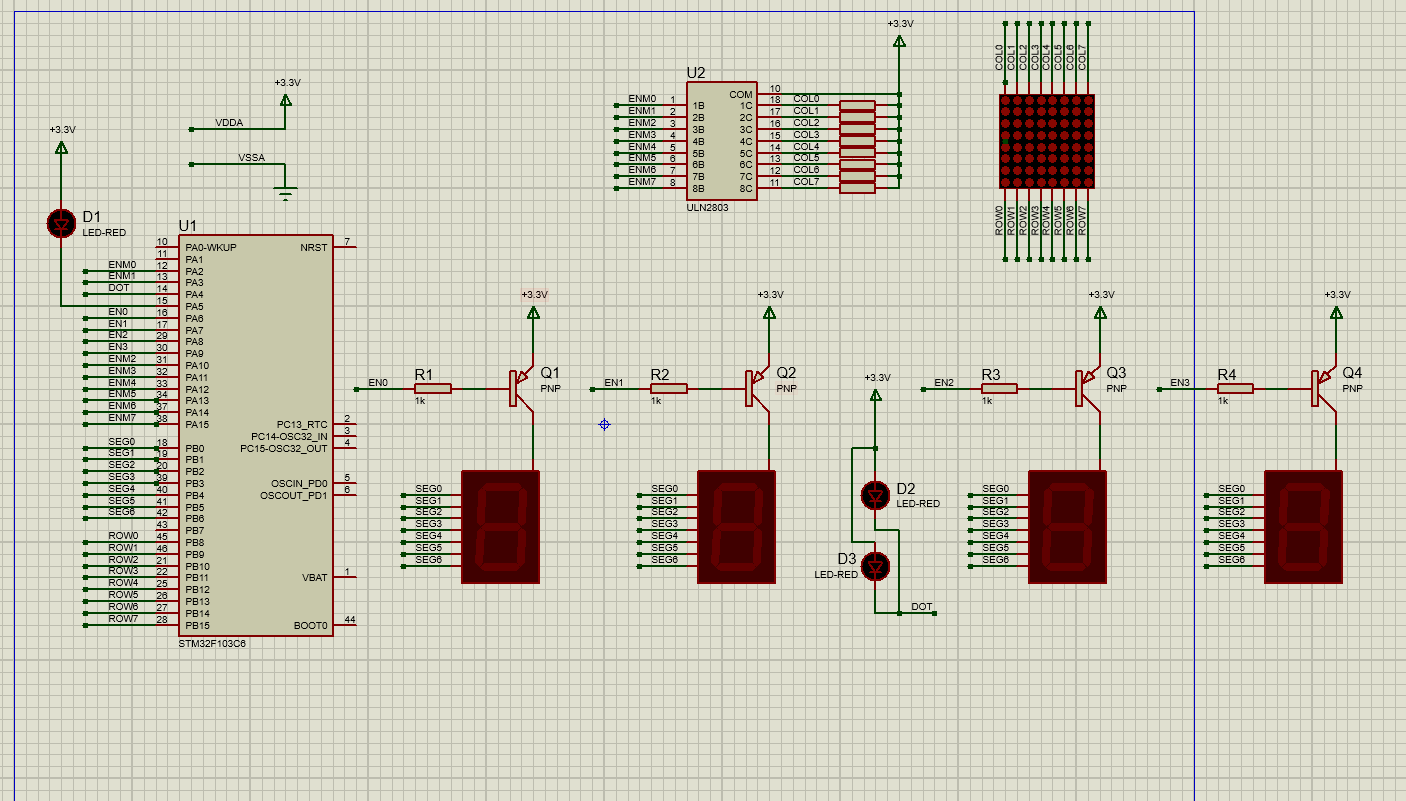
\includegraphics[width=\textwidth]{ex9.png}
\caption{Exercise 9: clock circuit with an eight-column LED matrix.}
\label{fig:ex9}
\end{figure}
In this circuit, a high ULN2803 input sinks its column node low and disables
that column. A low input releases the node, allowing its pull-up to select
the column. Selected row outputs are driven low to light pixels. Thus, the
application selects a column with a low ENM output. All columns are disabled
before changing row data, preventing the old column from receiving a new
pattern. GPIO pins used by debugging must be released for this mapping;
the matrix configuration uses PA13--PA15 as outputs.

\topic{Column buffer and row function}
The source uses one byte per column. Bit 0 corresponds to ROW0 and bit 7 to
ROW7; a one indicates a pixel to light. The character A is represented by
\code{{0x00, 0x7E, 0x09, 0x09, 0x09, 0x7E, 0x00, 0x00}}.
The two \code{0x7E} columns light rows 1--6, while \code{0x09} lights rows
0 and 3 for the top and crossbar. With ascending rows from top to bottom and
ascending columns from left to right, these patterns form A.
The binary forms explain the selected pixels directly:
\[
\texttt{0x7E}=\texttt{01111110}_{2},\qquad
\texttt{0x09}=\texttt{00001001}_{2}.
\]
Reading bits from bit zero upward, \code{0x7E} selects rows 1 through 6 and
\code{0x09} selects rows 0 and 3. Columns zero, six, and seven contain no
selected rows, leaving blank space around the character. The left and right
strokes use columns one and five, and columns two through four join those
strokes at the top and the crossbar.
\par\noindent\begin{minipage}{\linewidth}
\begin{lstlisting}[caption={Matrix definitions, buffer, and row output}]
#define ENM0_PIN GPIO_PIN_2
#define ENM1_PIN GPIO_PIN_3
#define ENM2_PIN GPIO_PIN_10
#define ENM3_PIN GPIO_PIN_11
#define ENM4_PIN GPIO_PIN_12
#define ENM5_PIN GPIO_PIN_13
#define ENM6_PIN GPIO_PIN_14
#define ENM7_PIN GPIO_PIN_15
#define ALL_ENM (ENM0_PIN | ENM1_PIN | ENM2_PIN | ENM3_PIN | \
                 ENM4_PIN | ENM5_PIN | ENM6_PIN | ENM7_PIN)
#define ALL_ROWS (GPIO_PIN_8 | GPIO_PIN_9 | GPIO_PIN_10 | \
                  GPIO_PIN_11 | GPIO_PIN_12 | GPIO_PIN_13 | \
                  GPIO_PIN_14 | GPIO_PIN_15)

const int MAX_LED_MATRIX = 8;
int index_led_matrix = 0;
uint8_t matrix_buffer[8] =
{
    0x00, 0x7E, 0x09, 0x09, 0x09, 0x7E, 0x00, 0x00
};

void setRow(int col)
{
    uint16_t row_data;

    row_data = (uint16_t)((uint16_t)matrix_buffer[col] << 8);
    HAL_GPIO_WritePin(GPIOB, ALL_ROWS, GPIO_PIN_SET);
    if (row_data != 0)
    {
        HAL_GPIO_WritePin(GPIOB, row_data, GPIO_PIN_RESET);
    }
}
\end{lstlisting}
\end{minipage}\par
The eight-bit pattern is shifted by eight positions because rows use the upper
half of GPIOB. The row mask and segment mask are disjoint, so row writes leave
the seven-segment pattern unchanged. The fixed-width types in these matrix
helpers store the byte pattern and GPIO mask used by HAL.
For example, column one contains \code{0x7E}. Shifting this byte left by
eight produces \code{0x7E00}, which corresponds to PB9--PB14. The first
GPIO write sets all row outputs high to clear the previous column pattern;
the second write drives only those selected row pins low. For a zero byte,
the second write is skipped, so the selected column remains blank.

\topic{Matrix selection function}
The selector disables all columns, validates the index, writes the required
rows, and enables exactly one column. An invalid index leaves the matrix blank.
The function follows the same separation used for seven-segment displays:
\code{setRow(index)} supplies the pixel data, and the switch case supplies
the physical column selection. Writing rows before enabling the next column
avoids briefly displaying its predecessor's pattern. Only the scanner advances
the index; the selection function itself prepares one column and returns.
\par\noindent\begin{minipage}{\linewidth}
\begin{lstlisting}[caption={updateLEDMatrix function}]
void updateLEDMatrix(int index)
{
    HAL_GPIO_WritePin(GPIOA, ALL_ENM, GPIO_PIN_SET);
    if (index < 0 || index >= MAX_LED_MATRIX)
    {
        return;
    }
    setRow(index);
    switch (index)
    {
        case 0:
            HAL_GPIO_WritePin(GPIOA, ENM0_PIN, GPIO_PIN_RESET);
            break;
        case 1:
            HAL_GPIO_WritePin(GPIOA, ENM1_PIN, GPIO_PIN_RESET);
            break;
        case 2:
            HAL_GPIO_WritePin(GPIOA, ENM2_PIN, GPIO_PIN_RESET);
            break;
        case 3:
            HAL_GPIO_WritePin(GPIOA, ENM3_PIN, GPIO_PIN_RESET);
            break;
        case 4:
            HAL_GPIO_WritePin(GPIOA, ENM4_PIN, GPIO_PIN_RESET);
            break;
        case 5:
            HAL_GPIO_WritePin(GPIOA, ENM5_PIN, GPIO_PIN_RESET);
            break;
        case 6:
            HAL_GPIO_WritePin(GPIOA, ENM6_PIN, GPIO_PIN_RESET);
            break;
        case 7:
            HAL_GPIO_WritePin(GPIOA, ENM7_PIN, GPIO_PIN_RESET);
            break;
        default:
            break;
    }
}
\end{lstlisting}
\end{minipage}\par

\topic{Foreground scheduling and scan timing}
Reuse timer2's declarations, setter, and countdown block from Exercise 6,
but assign it exclusively to matrix scanning in this version. Timer0 and
timer1 retain their Exercise 8 tasks. The callback remains the maintenance-only
callback, now calling the three-timer version of \code{timer_run()}.
Before the timer start in Exercise 8, add:
\par\noindent\begin{minipage}{\linewidth}
\begin{lstlisting}[caption={Matrix initialization before TIM2 starts}]
HAL_GPIO_WritePin(GPIOA, ALL_ENM, GPIO_PIN_SET);
HAL_GPIO_WritePin(GPIOB, ALL_ROWS, GPIO_PIN_SET);
updateLEDMatrix(0);
index_led_matrix = 1;
setTimer2(10);
\end{lstlisting}
\end{minipage}\par
Append the following independent expiry block to the Exercise 8 main loop:
\par\noindent\begin{minipage}{\linewidth}
\begin{lstlisting}[caption={Matrix scan task in main}]
if (timer2_flag == 1)
{
    setTimer2(10);
    updateLEDMatrix(index_led_matrix);
    index_led_matrix++;
    if (index_led_matrix >= MAX_LED_MATRIX)
    {
        index_led_matrix = 0;
    }
}
\end{lstlisting}
\end{minipage}\par
One column occupies one 10-ms slot. Eight columns form one complete frame:
\[
T_{\mathrm{frame}}=8\times10\ \mathrm{ms}=80\ \mathrm{ms},\qquad
f_{\mathrm{frame}}=12.5\ \mathrm{Hz}.
\]
The column-selection rate is 100 Hz, and the nominal duty cycle of each column
is one eighth. The expected image is the A pattern scanned repeatedly while
the clock continues running. At a 12.5-Hz frame rate, visible flicker can remain;
the column rate alone does not describe the refresh rate of the complete image.

\topic{Combining the matrix and clock tasks}
The new matrix timer loads one tick, whereas the digit timer loads 25 ticks
and the clock timer loads 100 ticks. On a typical 10-ms expiry, main handles
only the matrix task. At 250 ms, the digit and matrix tasks may both be ready;
at 1000 ms, all three tasks may be ready. The three independent flag checks
allow these events to be processed during one foreground iteration.

The initialization prepares column zero and sets the next index to one.
Under the nominal schedule, columns one through seven are then selected at
10, 20, 30, 40, 50, 60, and 70 ms. Column zero returns at 80 ms. Each column
is therefore revisited once every eight ticks. The clock and matrix use
separate buffers and GPIO masks, so updating the matrix rows does not erase
the numeral currently selected on the seven-segment display.

\section{Exercise 10: Left-shifting matrix animation}
\topic{Implementation idea: circular shifting}
The animation is created by changing display data rather than changing the
matrix scanning function. Each animation event rotates the eight column bytes
one position to the left. The outgoing first byte is inserted at the last
position, producing a continuous wraparound motion. The modification is made
only when column zero is about to be displayed so one frame never contains a
mixture of old and new column data.

This exercise reuses Figure~\ref{fig:ex9} and the matrix scanner. Moving each
column's data into the preceding buffer position shifts the pattern one column
left. The first column is saved and inserted at the right edge, so the animation
wraps around instead of discarding pixels. After eight shifts, the buffer
returns to its original arrangement.
For example, the initial buffer
\code{{0x00, 0x7E, 0x09, 0x09, 0x09, 0x7E, 0x00, 0x00}}
becomes
\code{{0x7E, 0x09, 0x09, 0x09, 0x7E, 0x00, 0x00, 0x00}}
after one left shift. The column data previously stored at position one is
now displayed at position zero. Saving the old first byte before the loop
prevents that outgoing column from being lost.

The loop copies from left to right. At iteration \code{i}, the old value
at \code{i + 1} has not yet been overwritten, so it can safely be copied
into position \code{i}. After positions zero through six have been updated,
the saved first byte is written into position seven. This performs one
circular shift without a second eight-byte buffer.

Timer3 requests a shift after 200 ms. The shift is applied only when the next
column index is zero, immediately before a new frame begins. This keeps one
buffer arrangement for all eight columns of a frame.
\par\noindent\begin{minipage}{\linewidth}
\begin{lstlisting}[caption={Animation timer and circular shift helper}]
int timer3_counter = 0;
int timer3_flag = 0;

void setTimer3(int duration)
{
    timer3_counter = duration / TIMER_CYCLE;
    timer3_flag = 0;
}

void shiftMatrixLeft(void)
{
    int i;
    uint8_t first_column;

    first_column = matrix_buffer[0];
    for (i = 0; i < MAX_LED_MATRIX - 1; i++)
    {
        matrix_buffer[i] = matrix_buffer[i + 1];
    }
    matrix_buffer[MAX_LED_MATRIX - 1] = first_column;
}
\end{lstlisting}
\end{minipage}\par
Append this block inside \code{timer_run()} after the first three countdowns:
\par\noindent\begin{minipage}{\linewidth}
\begin{lstlisting}[caption={Animation countdown maintenance}]
if (timer3_counter > 0)
{
    timer3_counter--;
    if (timer3_counter == 0)
    {
        timer3_flag = 1;
    }
}
\end{lstlisting}
\end{minipage}\par
Arm \code{setTimer3(200)} before starting TIM2. Replace the matrix expiry
block from Exercise 9 with the following block; the clock and digit tasks
remain unchanged:
\par\noindent\begin{minipage}{\linewidth}
\begin{lstlisting}[caption={Frame-aligned animation task in main}]
if (timer2_flag == 1)
{
    setTimer2(10);
    if (index_led_matrix == 0 && timer3_flag == 1)
    {
        setTimer3(200);
        shiftMatrixLeft();
    }
    updateLEDMatrix(index_led_matrix);
    index_led_matrix++;
    if (index_led_matrix >= MAX_LED_MATRIX)
    {
        index_led_matrix = 0;
    }
}
\end{lstlisting}
\end{minipage}\par

\topic{Animation interval and expected behavior}
The request interval is 20 hardware ticks, or 200 ms. However, the code does
not shift immediately at expiry: it waits for a column-zero boundary. With
ideal 10-ms column slots, frame boundaries occur every 80 ms. Because timer3
is rearmed at the actual shift, the next eligible boundary after 200 ms is
reached after three complete frames. Two frames take only 160 ms, whereas
three frames take 240 ms:
\[
T_{\mathrm{shift}}=
\left\lceil\frac{200}{80}\right\rceil\times80
=240\ \mathrm{ms}.
\]
The expected steady motion is therefore approximately one column every
240 ms, rather than exactly every 200 ms. Eight shifts take approximately
\(8\times240=1920\) ms. These are nominal intervals derived from the scheduled
scan; foreground processing can affect the exact event times. Increasing the
timer3 duration slows the movement. The matrix frame rate remains 12.5 Hz
because timer2's 10-ms scan interval is unchanged.

\topic{Pending request and first animation step}
The initial matrix column is zero, with the next index set to one. Its next
column-zero boundaries occur at approximately 80, 160, and 240 ms. Timer3
expires at 200 ms, while the matrix is between frame boundaries. The shift
condition is therefore false even though \code{timer3_flag} is one. The flag
remains set until a later matrix event begins with index zero.

At 240 ms, both requirements are met: the matrix scan timer has expired and
the next column is zero. Main reloads timer3, shifts the buffer, and then
displays column zero from the new arrangement. Columns one through seven
subsequently use that same arrangement. The next request becomes ready at
approximately 440 ms and is applied at the 480-ms frame boundary. This trace
explains why the selected code produces nominal 240-ms motion steps while
retaining the 200-ms request duration.

\section*{Conclusion}
\addcontentsline{toc}{section}{Conclusion}
The laboratory demonstrates how shared segment signals and individual enable
outputs implement multiplexed displays. The complete scanning frequency depends
on both the slot duration and the number of selected digits or columns. A
10-ms timer interrupt provides a common base for independent software timers,
allowing one-second clock updates, DOT transitions, digit selection, matrix
refresh, and animation to use different intervals.

Decimal buffer conversion separates time representation from display control,
including leading zeros and day rollover. Replacing the blocking clock delay
with counter-and-flag timing keeps the main loop available for other tasks.
Moving digit scanning and matrix processing into main further reduces interrupt
work to timer maintenance. Finally, circular buffer shifting and frame-boundary
updates combine repeated matrix scanning with coherent character animation.
\clearpage
\phantomsection
\addcontentsline{toc}{section}{References}
\begin{thebibliography}{4}
\bibitem{stm32}
STMicroelectronics, ``STM32F103 product family,'' product documentation.
Available from the
\href{https://www.st.com/en/microcontrollers-microprocessors/stm32f103.html}
{STMicroelectronics STM32F103 product page}.
Accessed: October 5, 2026.

\bibitem{hal}
STMicroelectronics, \emph{Description of STM32F1 HAL and Low-Layer Drivers},
User Manual UM1850. Available from the
\href{https://www.st.com/resource/en/user_manual/um1850-description-of-stm32f1-hal-and-lowlayer-drivers-stmicroelectronics.pdf}
{STMicroelectronics document archive}.
Accessed: October 5, 2026.

\bibitem{keil}
Arm Keil, ``\mbox{$\mu$Vision} User's Guide.'' Available from the
\href{https://www.keil.com/support/man/docs/uv4/default.htm}
{Keil documentation website}.
Accessed: October 5, 2026.

\bibitem{proteus}
Labcenter Electronics, ``Proteus Design Suite: PCB design and circuit simulation
software.'' Available from the
\href{https://www.labcenter.com/}{Labcenter Electronics website}.
Accessed: October 5, 2026.
\end{thebibliography}
\end{document}
